\documentclass[12pt]{article}

\usepackage[a1paper,portrait,margin=16mm]{geometry}
\usepackage[T1]{fontenc}
\usepackage[utf8]{inputenc}
\usepackage{lmodern}
\usepackage{microtype}
\usepackage{graphicx}
\usepackage{booktabs}
\usepackage[table]{xcolor}
\usepackage{array}
\usepackage{multicol}
\usepackage{enumitem}
\usepackage[hidelinks]{hyperref}

\setlength{\columnsep}{14mm}
\setlength{\parindent}{0pt}
\setlength{\parskip}{0.58em}
\setlength{\tabcolsep}{7pt}
\renewcommand{\arraystretch}{1.16}
\pagestyle{empty}

\AtBeginDocument{\fontsize{14.5}{17.5}\selectfont}

\definecolor{PosterBlue}{RGB}{13,58,92}
\definecolor{PosterTeal}{RGB}{27,121,140}
\definecolor{PosterGray}{RGB}{243,246,248}
\definecolor{PosterLine}{RGB}{210,218,224}
\definecolor{PosterMint}{RGB}{216,238,224}
\definecolor{PosterGold}{RGB}{247,232,193}
\definecolor{PosterRose}{RGB}{247,220,220}
\definecolor{PosterSky}{RGB}{219,233,244}
\definecolor{PosterLavender}{RGB}{232,223,247}
\definecolor{PosterApricot}{RGB}{246,224,207}
\definecolor{PosterAqua}{RGB}{210,236,239}

\arrayrulecolor{PosterLine}

\newcommand{\postersection}[1]{%
  \vspace{0.48em}
  {\color{PosterBlue}\rule{\linewidth}{1.5pt}}\par
  \vspace{0.38em}
  {\fontsize{21}{25}\selectfont\bfseries\color{PosterBlue} #1}\par
  \vspace{0.24em}
}

\newcommand{\takeawaybox}[1]{%
  \setlength{\fboxsep}{12pt}%
  \colorbox{PosterGray}{%
    \parbox{0.97\linewidth}{\bfseries\fontsize{16.5}{20}\selectfont #1}%
  }%
}

\newcommand{\highlightbox}[2]{%
  \setlength{\fboxsep}{9pt}%
  \colorbox{PosterGray}{%
    \parbox{0.97\linewidth}{\fontsize{14}{17}\selectfont\textbf{#1} #2}%
  }%
}

\newcommand{\takeawayspanel}[1]{%
  \setlength{\fboxsep}{10pt}%
  \fcolorbox{PosterTeal}{PosterBlue!4}{%
    \parbox{0.955\linewidth}{#1}%
  }%
}

\newcommand{\headerrow}{\rowcolor{PosterBlue!12}}
\newcommand{\best}[1]{\cellcolor{PosterMint}\textbf{#1}}
\newcommand{\good}[1]{\cellcolor{PosterMint}#1}
\newcommand{\warn}[1]{\cellcolor{PosterGold}#1}
\newcommand{\hardcase}[1]{\cellcolor{PosterRose}#1}
\newcommand{\lexicon}[1]{\cellcolor{PosterLavender}\textbf{#1}}
\newcommand{\classical}[1]{\cellcolor{PosterApricot}\textbf{#1}}
\newcommand{\transformer}[1]{\cellcolor{PosterSky}\textbf{#1}}
\newcommand{\llm}[1]{\cellcolor{PosterAqua}\textbf{#1}}
\newcommand{\deep}[1]{\cellcolor{PosterGold}\textbf{#1}}
\newcommand{\llmstrategy}[1]{\cellcolor{PosterAqua}\textbf{#1}}
\newcommand{\crossstrategy}[1]{\cellcolor{PosterMint}\textbf{#1}}
\newcommand{\cascadestrategy}[1]{\cellcolor{PosterGold}\textbf{#1}}

\begin{document}

\twocolumn[
\begin{center}
{\fontsize{31}{36}\selectfont\bfseries Benchmarking Classical ML, Transformers, and Large Language Models in Multidomain Sentiment Classification\par}
\vspace{0.7em}
{\fontsize{19}{23}\selectfont Michal Szlązak, Krzysztof Jurkowski, Arkadiusz Ciepliński, Marek Wdowiak\par}
\vspace{0.3em}
{\fontsize{16.5}{20}\selectfont Warsaw University of Technology\par}
\vspace{0.9em}
\takeawaybox{No single sentiment model dominates across all domains. The strongest practical systems are domain-aware and combine heterogeneous models through voting or confidence-based routing.}
\vspace{1.2em}
\end{center}
]

\postersection{Introduction}
Sentiment analysis remains useful in opinion mining, customer feedback, finance, and social media monitoring, but model quality depends strongly on domain, label scheme, text length, and linguistic ambiguity. A system that works well on long movie reviews may fail on short tweets, irony, or formal financial statements.

This work compares classical ML, deep learning, transformers, and large language models across a multidomain benchmark. We also evaluate whether voting and confidence-based hybrid pipelines can improve accuracy without depending entirely on the most expensive model.

The goal of the study is not only to rank models, but also to understand \emph{why} some combinations work. In particular, we ask whether stronger results come from model scale alone, or from combining model families with complementary error profiles.

This study asks two practical questions:
\begin{itemize}[leftmargin=1.2em,itemsep=0.3em,topsep=0.3em]
  \item Is there one model family that works best across all sentiment domains?
  \item Can voting and hybrid pipelines improve quality without relying on one expensive model?
\end{itemize}

\highlightbox{Research question.}{Which model families work best across domains, and when do hybrid strategies actually help?}

\postersection{Datasets}
We evaluate six public benchmarks spanning finance, reviews, and social media, which together yield nine experimental configurations.

\begin{center}
\rowcolors{2}{PosterBlue!4}{white}
\begin{tabular}{>{\raggedright\arraybackslash}p{0.38\linewidth} >{\raggedright\arraybackslash}p{0.29\linewidth} >{\centering\arraybackslash}p{0.12\linewidth} >{\raggedleft\arraybackslash}p{0.13\linewidth}}
\toprule
\headerrow
\textbf{Dataset} & \textbf{Domain} & \textbf{Classes} & \textbf{Test size} \\
\midrule
IMDB & Movie reviews & 2 & 10,000 \\
Financial PhraseBank & Financial news & 3 & varies \\
Twitter Entity & Social media & 4 & 15,000 \\
TweetEval Sentiment & Social media & 3 & 15,000 \\
TweetEval Irony & Social media & 2 & 1,800 \\
Yelp Full & Reviews & 5 & 5,000 \\
\bottomrule
\end{tabular}
\end{center}

The benchmark intentionally mixes clean and noisy text, binary and multi-class settings, as well as explicit and subtle sentiment. This allows us to test not only average accuracy, but also robustness under very different linguistic conditions.

\begin{center}
\rowcolors{2}{PosterBlue!4}{white}
\begin{tabular}{>{\raggedright\arraybackslash}p{0.27\linewidth} >{\raggedright\arraybackslash}p{0.29\linewidth} >{\raggedright\arraybackslash}p{0.34\linewidth}}
\toprule
\headerrow
\textbf{Benchmark group} & \textbf{Main challenge} & \textbf{Why it matters} \\
\midrule
Finance subsets & domain-specific phrasing, label ambiguity & tests sensitivity to annotation quality and expert language \\
IMDB & long-form reasoning & tests sentiment over extended narrative text \\
Twitter / TweetEval & short, noisy, context-poor messages & tests robustness to slang, fragmentation, and irony \\
Yelp Full & 5-class rating prediction & tests fine-grained sentiment discrimination \\
\bottomrule
\end{tabular}
\end{center}

\postersection{Models and Single-Model Results}
We compare nine models from five families and first evaluate them as standalone classifiers.
\begin{itemize}[leftmargin=1.2em,itemsep=0.3em,topsep=0.3em]
  \item Lexicon-based: VADER
  \item Classical ML: TF-IDF + SVM
  \item Deep learning: CNN, LSTM
  \item Transformers: DistilBERT, DistilRoBERTa
  \item LLMs: Gemini, Mistral, Llama
\end{itemize}

All models are evaluated with Accuracy and Macro-F1. The main pattern is domain sensitivity: different datasets prefer different model families.

Classical and shallow neural models remain competitive on some noisy benchmarks, while fine-tuned transformers dominate finance. LLMs are strongest when longer context or more implicit reasoning is needed, but they are not universally superior.

\begin{center}
\rowcolors{2}{PosterBlue!4}{white}
\begin{tabular}{>{\raggedright\arraybackslash}p{0.23\linewidth} >{\raggedright\arraybackslash}p{0.23\linewidth} >{\raggedright\arraybackslash}p{0.42\linewidth}}
\toprule
\headerrow
\textbf{Family} & \textbf{Models} & \textbf{Typical strength in this benchmark} \\
\midrule
\lexicon{Lexicon-based} & VADER & lightweight baseline with no training, but weakest on complex multi-class tasks \\
\classical{Classical ML} & TF-IDF + SVM & strong on structured text, competitive on finance and IMDB \\
\deep{Deep learning} & CNN, LSTM & effective on short and noisy social media data, especially Twitter \\
\transformer{Transformers} & DistilBERT, DistilRoBERTa & strongest supervised models overall, especially in finance \\
\llm{LLMs} & Gemini, Mistral, Llama & strongest on IMDB and irony, flexible without task-specific fine-tuning \\
\bottomrule
\end{tabular}
\end{center}

\begin{center}
\rowcolors{2}{PosterBlue!4}{white}
\begin{tabular}{>{\raggedright\arraybackslash}p{0.38\linewidth} >{\raggedright\arraybackslash}p{0.35\linewidth} >{\centering\arraybackslash}p{0.16\linewidth}}
\toprule
\headerrow
\textbf{Dataset} & \textbf{Best single model} & \textbf{Accuracy} \\
\midrule
Finance-50 & \transformer{DistilRoBERTa} & 0.865 \\
Finance-66 & \transformer{DistilRoBERTa} & 0.884 \\
Finance-75 & \transformer{DistilRoBERTa} & 0.938 \\
Finance-All & \transformer{DistilRoBERTa} & \best{0.971} \\
IMDB & \llm{Gemini} & \good{0.958} \\
TE-Irony & \llm{Gemini} & 0.809 \\
TE-Sentiment & \transformer{DistilRoBERTa} & 0.707 \\
Twitter & \deep{CNN} & 0.866 \\
Yelp-Full & \llm{Mistral} & 0.666 \\
\bottomrule
\end{tabular}
\end{center}

Several individual results are especially informative. DistilRoBERTa reaches 0.971 on Finance-All and remains the strongest single model on all four finance subsets. Gemini reaches 0.958 on IMDB and 0.809 on TweetEval-Irony, showing that LLMs can be most effective on linguistically complex tasks. On Twitter, however, CNN reaches 0.866 and clearly outperforms all LLMs, which confirms that noisy short-form text often favors more task-specific architectures.

\highlightbox{Main observation.}{No single model family dominates across all datasets: transformers lead in finance, LLMs are strongest on IMDB and irony, while CNN-based models perform best on Twitter.}

\postersection{Voting and Hybrid Strategies}
After benchmarking single models, we test whether combining predictions improves robustness.

\begin{itemize}[leftmargin=1.2em,itemsep=0.3em,topsep=0.3em]
  \item LLM-only voting: Gemini, Mistral, and Llama vote on the final label.
  \item Confidence-based cascade: SVM $\rightarrow$ CNN $\rightarrow$ LSTM $\rightarrow$ DistilRoBERTa $\rightarrow$ Gemini.
  \item Cross-model voting: majority and confidence-weighted aggregation across all model families.
\end{itemize}

The most reliable ensemble strategy is confidence-weighted voting, while Twitter is the clearest example that not every model should always be included. The hybrid cascade with a 0.90 confidence threshold gives the most stable quality-cost trade-off across datasets.

\begin{center}
\highlightbox{Cascade.}{TF-IDF + SVM $\rightarrow$ CNN $\rightarrow$ LSTM $\rightarrow$ DistilRoBERTa $\rightarrow$ Gemini}
\end{center}

\begin{center}
\rowcolors{2}{PosterBlue!4}{white}
\begin{tabular}{>{\raggedright\arraybackslash}p{0.28\linewidth} >{\raggedright\arraybackslash}p{0.27\linewidth} >{\raggedright\arraybackslash}p{0.29\linewidth}}
\toprule
\headerrow
\textbf{Strategy} & \textbf{Core idea} & \textbf{Main takeaway} \\
\midrule
\llmstrategy{LLM-only voting} & combine Gemini, Mistral, and Llama & \llmstrategy{small gains on selected datasets, especially finance} \\
\crossstrategy{Cross-model voting} & aggregate all model families & \crossstrategy{best when errors are complementary} \\
\cascadestrategy{Confidence cascade} & route easy cases to cheaper models & \cascadestrategy{improves the cost-quality trade-off in practice} \\
\bottomrule
\end{tabular}
\end{center}

\begin{center}
\rowcolors{2}{PosterBlue!4}{white}
\begin{tabular}{>{\raggedright\arraybackslash}p{0.34\linewidth} >{\centering\arraybackslash}p{0.19\linewidth} >{\centering\arraybackslash}p{0.18\linewidth} >{\centering\arraybackslash}p{0.19\linewidth}}
\toprule
\headerrow
\textbf{Dataset} & \textbf{Best single} & \textbf{Ensemble} & \textbf{Delta} \\
\midrule
Finance-66 & 0.884 & 0.912 & \best{+0.028} \\
Finance-75 & 0.938 & 0.964 & \good{+0.026} \\
Finance-All & 0.971 & 0.980 & \good{+0.009} \\
IMDB & 0.958 & 0.959 & \good{+0.001} \\
Twitter & 0.866 & 0.891* & \good{+0.025} \\
Yelp-Full & 0.666 & 0.659 & \hardcase{-0.007} \\
\bottomrule
\end{tabular}

\vspace{0.3em}
{\small * Majority voting without LLMs was best on Twitter.}
\end{center}

The cross-model results show that confidence-weighted voting is the most reliable ensemble strategy, producing the best result on eight of nine datasets and reaching gains of up to +2.8 percentage points relative to the best single model. The exception is Twitter, where excluding LLMs from majority voting produces the strongest ensemble because the three generative models underperform the CNN and LSTM baselines on that dataset.

The hybrid cascade tells a slightly different story. Threshold 0.98 sometimes gives the highest accuracy, but it is unstable and routes many more samples to the final expensive model. Threshold 0.90 is therefore the most practical operating point: it preserves competitive accuracy while offloading a large share of examples to cheaper models earlier in the pipeline.

\postersection{Error Analysis}
Error analysis explains why some combinations help and others do not. Models from the same family often fail on the same samples, so adding more similar models does not automatically improve diversity.

Across all datasets, mean Jaccard overlap of error sets is 0.414 for within-family pairs and 0.234 for cross-family pairs. This is why heterogeneous ensembles are more useful than simply stacking more models of one type.

\begin{center}
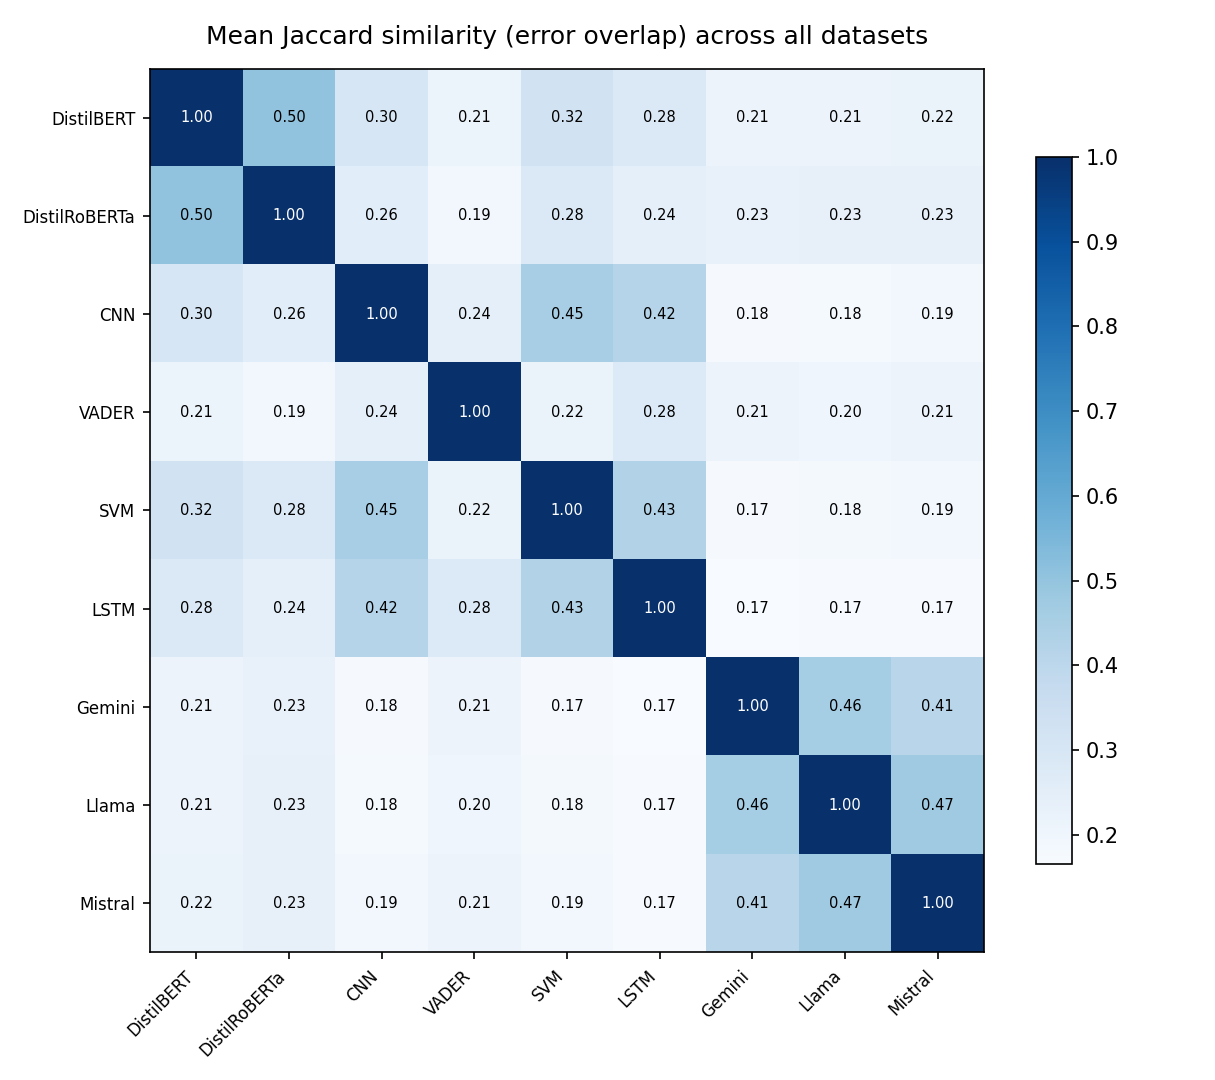
\includegraphics[width=0.92\linewidth]{../data/mean_pairwise_jaccard.png}

{\small Mean pairwise Jaccard overlap of model error sets. Darker cells indicate more similar failure patterns.}
\end{center}

The overlap structure is not only a descriptive result. It explains why adding more models from the same family often yields limited gains: transformer-transformer and LLM-LLM pairs tend to fail on many of the same examples. Ensemble improvements are therefore larger when the pool mixes families with genuinely different failure modes.

\begin{center}
\rowcolors{2}{PosterBlue!4}{white}
\begin{tabular}{>{\raggedright\arraybackslash}p{0.26\linewidth} >{\centering\arraybackslash}p{0.16\linewidth} >{\centering\arraybackslash}p{0.16\linewidth} >{\centering\arraybackslash}p{0.16\linewidth} >{\centering\arraybackslash}p{0.16\linewidth}}
\toprule
\headerrow
\textbf{Dataset} & \textbf{Within} & \textbf{Between} & \textbf{Hard \%} & \textbf{All-fail \%} \\
\midrule
Finance-All & 0.308 & 0.106 & \best{1.10} & \best{0.00} \\
IMDB & 0.372 & 0.178 & 2.62 & 0.50 \\
TE-Sentiment & 0.519 & 0.344 & \warn{21.39} & \warn{3.37} \\
Yelp-Full & \hardcase{0.556} & \hardcase{0.429} & \hardcase{32.84} & \hardcase{7.88} \\
\bottomrule
\end{tabular}
\end{center}

Dataset difficulty is equally important. Finance-All contains relatively few hard or universally misclassified examples, which makes it easier to improve through aggregation. In contrast, Yelp-Full and TweetEval-Sentiment contain many samples that are hard for nearly every model. These cases often involve mixed polarity, sarcasm, understatement, or fine-grained rating decisions rather than simple positive-negative sentiment.

The broader implication is that fixed voting has a real ceiling. When most architectures fail on the same sample, simple majority aggregation has little corrective power. This is why the most promising next step is not just building larger ensembles, but designing more selective domain-aware hybrids.

\postersection{Key Takeaways}
\takeawayspanel{%
{\color{PosterBlue}\bfseries\fontsize{17}{20}\selectfont Main conclusions}\par
\vspace{0.35em}
\begin{itemize}[leftmargin=1.2em,itemsep=0.34em,topsep=0.2em]
  \item \textbf{No single architecture is optimal across all domains.}
  \item \textbf{Finance datasets prefer transformers,} while IMDB and irony favour LLMs, and Twitter favours CNN/LSTM models.
  \item \textbf{Confidence-weighted voting is the most reliable ensemble strategy} across datasets.
  \item \textbf{A 0.90 confidence threshold gives the best practical balance} between quality and computational cost.
  \item \textbf{Hard examples and correlated errors limit what fixed voting can achieve.}
\end{itemize}%
}

\textbf{Scientific contribution.} The study combines a unified multidomain comparison of five model families with a practical evaluation of three hybrid strategies and an error-overlap analysis that explains when aggregation can and cannot help.

\vfill

{\small
\textbf{Demo note.} This poster follows a simplified two-column structure derived from the article in \texttt{paper/IEEE-conference-template-062824.tex}. It is intended as a concise conference-poster version of the full paper.
}

\end{document}